\section{Online {\IterComp} Overview} \label{sec:oic-infra}

Although {\itercomp} had been originally proposed as an \textit{offline} optimization strategy, it can be adapted to work in
\textit{online} scenarios. Instead of selecting the best optimization sequence at development time, a first version of the program is
shipped bundled with the {\itercomp} mechanism. Our mechanism produces new application binaries using different optimization sequences.
When the user starts the application, we load and execute one of these binaries to evaluate the corresponding sequence online. Our
mechanism operates on the application's Intermediate Representation (IR) produced by LLVM. This saves us the effort of repeatedly parsing
the code through the frontend and removes the need for shipping the full application code.

\begin{figure}[t]
    \centering
    \includegraphics[width=\linewidth]{figs/infra-diagram}
    \caption{Overview of the online \itercomp mechanism. \red{zw: mark the boundary of online and offline.}}
    \label{fig:infra-diagram}
\end{figure}

Figure~\ref{fig:infra-diagram} shows an overview of how our online {\itercomp} mechanism works. On the developer's side, the program is
pre-compiled to IR without optimizations and is instrumented to measure the amount of work performed and the wall-clock time. On the user's
side, we select an optimization sequence and then compile the instrumented IR to binary using this sequence. Next time the user runs the
application, we measure the work and the execution time. We accumulate multiple such measurements until we can estimate the efficiency
metric P of this optimization sequence with high confidence. Finally, we use this information to help us select the next optimization
sequence.

This work focuses on the highlighted components of Figure~\ref{fig:infra-diagram}. The first one, \textit{Work Instrumentation} \blue{is
performed once at offline compile time}. It allows measuring the amount of work performed. Conceptually, we use the cost model of
Section~\ref{sec:metric} to estimate a cost for each basic block of the IR and then add instrumentation to increase a global work counter
by that cost every time a basic block is executed. The measured work should depend only on the program and the input, not the applied
optimizations, so we instrument the unoptimized IR before any optimizations modify it. We present a detailed description of work
instrumentation and how to keep it lightweight in Section~\ref{chap:instr}.

\textit{Optimization Selector} is responsible for selecting which optimization sequence to use for the next execution of the program. Each
sequence is used for multiple executions of the program in order to gather enough work efficiency measurements. When we are able to
estimate this work efficiency with a confidence interval narrower than a certain threshold, we can start evaluating a different
optimization sequence. We call the number of executions performed using the same optimization sequence the \textit{Input-Window Size}.

%\FIXME{WHAT IS THE OPTIMIZATION EVALUATOR? WHY IS IT HIGHLIGHTED? DO WE HAVE ANYTHING TO SAY ABOUT IT?}

\subsection{Efficient Optimization Selection and Compilation}

Most devices have distinct idle and peak usage periods. For example, mobile devices are used intensely during the day and not at all while
the user is sleeping and the battery is charging~\citep{mpeis16}. Many researchers have identified similar idle and peak usage periods in
the context of data centers~\citep{armbrust10,chen12b}. The proposed \itercomp infrastructure is very well suited to such scenarios. In
particular, we can use periods of idleness or underutilization to select the next few optimization sequences to try and compile the
corresponding binaries. This approach effectively hides the compilation overhead from the user. During peak periods, we only have to select
which of the existing binaries to evaluate which introduces almost no overhead.
